\subsection{Ca sử dụng chia sẻ vị trí}
\vspace{0.5cm}


\noindent 
\begin{tabularx}{\linewidth}{| l | X |} 
\hline 
\textbf{Mô tả} & Người dùng trong cùng chuyến đi có thể chia sẻ vị trí khi chuyến đi dang diễn ra. \\
\hline 
\textbf{Luồng cơ bản} & 1. Người dùng chọn một chuyến đi đang diễn ra. \newline
                        2. Hệ thống lây dữ liệu chi tiết của chuyến đi và hiển thị. \newline
                        3. Người dùng bấm "Chia sẻ vị trí". \newline
                        4. Hệ thống điều hường người dùng ra trang hiển thị bản đồ. \newline
                        5. Hệ thống cập nhật liên tục trong thời gian thực vị trí của bản thân người dùng và các người dùng khác tham gia. \\
             
               
% \hline 
% \textbf{Luồng thay thế} & Chuyến đi không đủ thông tin hệ thống sẽ thông báo lỗi chưa đủ thông tin. \\
       
\hline 
\textbf{Tiền điều kiện} & - Người dùng đang đăng nhập và phiên đăng nhập chưa kết thúc.\newline
                        - Người dùng đã tạo hoặc tham gia ít nhất một chuyến đi. \newline
                        - Chuyến đi đang trong trạng thái "Đang diễn ra".\\


\hline 
\textbf{Hậu điều kiện} & - Hệ thống cập nhật vị trí của người dùng và các người dùng khác trong chuyến đi. \newline
- Hệ thống hiển thị vị trí của người dùng và các người dùng khác trên bản đồ. \newline
- Hệ thống tạo thông báo đẩy trong thiết bị để chạy nền tác vụ \\
                        

\hline 
\textbf{Yêu cầu phi chức năng} & Hệ thống công khai chuyến đi dưới 2s \\
\hline 
\end{tabularx}

\noindent 
\begin{tabular}{| c | c |}
    \hline
    \textbf{Biểu đồ hoạt động} & \textbf{Quan hệ} \\ 
    \hline
    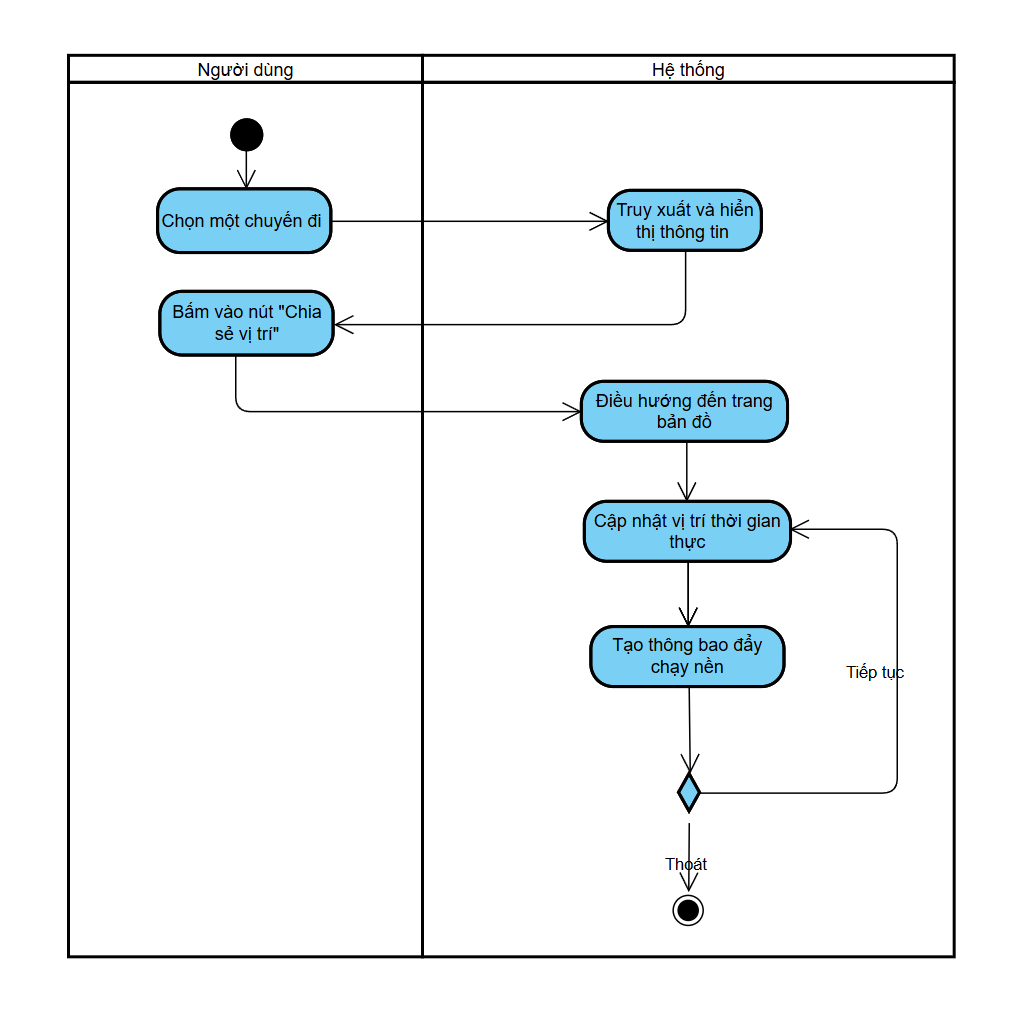
\includegraphics[width=0.5\linewidth]{figures/c3/3-3-16-ad.png} 
    & 
    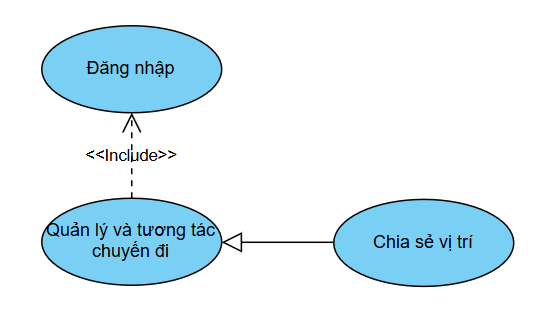
\includegraphics[width=0.45\linewidth]{figures/c3/3-3-16-rd.png} \\ 
    \hline
\end{tabular}

\vspace{0.8cm}

\begin{figure}[H]
    \centering  
    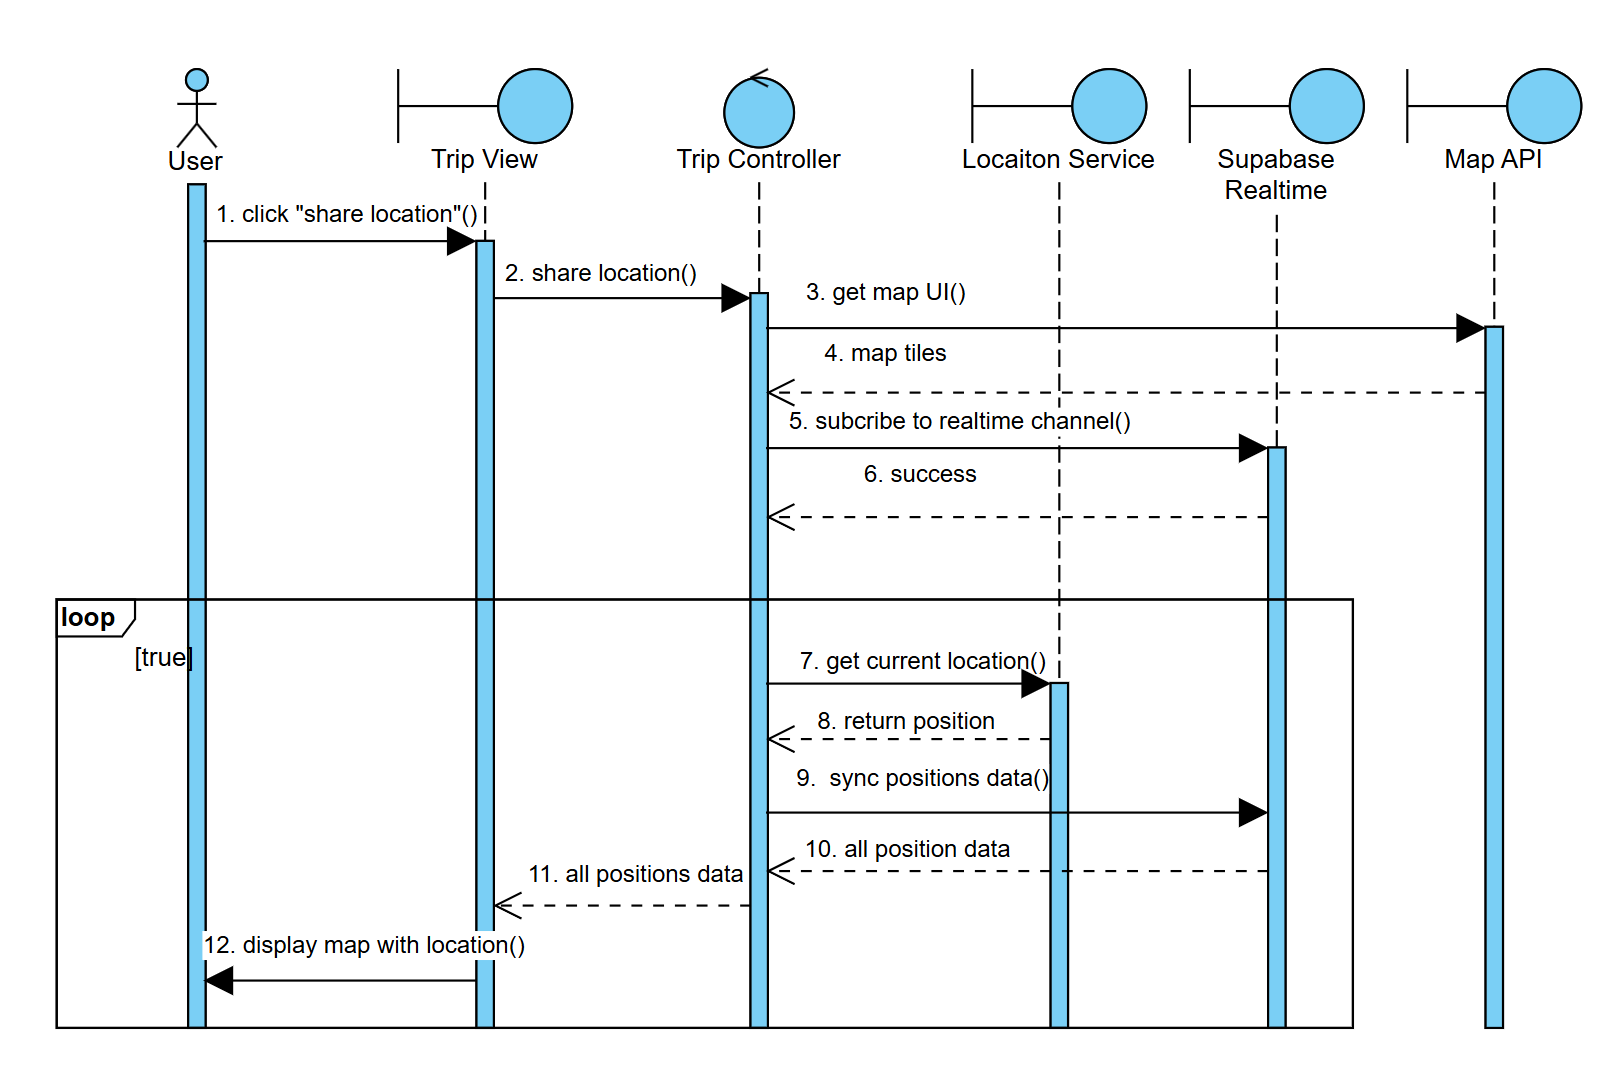
\includegraphics[width=1\textwidth]{figures/c3/3-3-16-sd.png}
    \caption{Biểu đồ tuần tự ca sử dụng chia sẻ vị trí.}
    \label{fig:3-3-16-sequence-diagram}
\end{figure}